\documentclass[
  11pt,
  letterpaper,
   addpoints,
   %answers
  ]{exam}

\usepackage{../exercise-preamble}

\begin{document}

\noindent
\begin{minipage}{0.47\textwidth}

\includegraphics[width=\textwidth]{../fcfm_die}
\end{minipage}
\begin{minipage}{0.53\textwidth}
\begin{center} 
\large\textbf{Fundamentos de control de sistemas} (EL4111-1) \\
\large\textbf{Ejercicio 1} \\
\small Prof.~Roberto Cardenas Dobson\\
\small Prof.~Aux.~Osvaldo Jimenez - Erik Sáez\\
\small Ayudantes.~Simon Arenas- Juan Pablo Baez - Francisco Garces - Sofia Ibarra\\
\end{center}
\end{minipage}

\vspace{0.5cm}
\noindent
\vspace{.85cm}
\hrule
\textbf{Instrucciones: La tarea debe ser entregada en formato digital(o escaneado) y legible (PDF) a través de U-Cursos. La fecha de entrega es el día 1 de Septiembre a las 23:59 hrs. No se aceptarán entregas atrasadas.}
\hrule
\begin{questions}
    %%%%%%%%%%%%%%%%%%%%%%%%%%%
    \question Un sistema tiene la siguiente planta:
    \begin{align*}
        H(s)G(s) = \frac{(s+a)}{s^{2}-2as+a^{2}}
    \end{align*}
    Donde a es una variable que depende de la potencia nominal de la planta y que se puede asumir como un valor de diseño. Un diseñador con poca experiencia decide utilizar un lazo de realimentación unitario y un controlador proporcional
    \begin{enumerate}
        \item Utilizando las condiciones de módulo y/o ángulo, en forma gráfica, plantee el problema y determine el rango de ganancia proporcional que produce inestabilidad.
        \item El diseñador añade un nuevo requerimiento al sistema de control: el tiempo de establecimiento del 2\%, definido como \(\frac{4}{\omega \zeta}\), debe ser igual a \(\frac{4}{a}\). Utilizando las condiciones de módulo y/o ángulo, en forma gráfica, determine la ganancia proporcional que entrega el tiempo de establecimiento solicitado.
        \item Para la pregunta (b), encuentre la frecuencia natural y el coeficiente de amortiguamiento obtenido con la solución propuesta.
    \end{enumerate}
    
    %%%%%%%%%%%%%%%%%%%%%%%%%%%
   
    %%%%%%%%%%%%%%%%%%%%%%%%%%%
    \question Sea el siguiente diagrama:
    \begin{figure}[h]
        \centering
        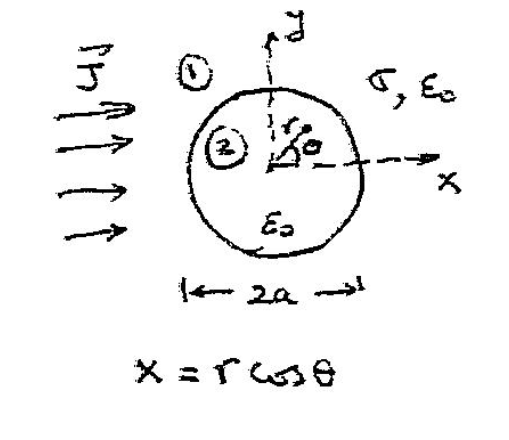
\includegraphics[width=0.5\textwidth]{Ejercicio_1_1}
    \end{figure}
    \begin{enumerate}
        \item Considerando el sistema de la Figura, tal que $G_{c}(s) = K$ y $G_{p}(s) = \frac{1}{s(s+2)(s+3)(s+9)}$ . Determine para que condiciones de $K>0$ el lazo cerrado es estable.
        \item En que varia su sistema si la ganancia $K<0$ , explique y demueestre graficamente
    \end{enumerate}
%%%%%%%%%%%%%%%%%%%%%%%%%%%
%%%%%%%%%%%%%%%%%%%%%%%%%%%
\end{questions}
\newpage
%%%%%%%%%%%%%%%%%%%%%%%%%%%

\end{document}